\title{Taler: Usable, privacy-preserving payments for the Web}

% Not sure how to do authors with the
% IEEEtran template correctly ...
\author{%
Jeffrey Burdges\and \\
Florian Dold\and \\
Christian Grothoff\and \\
Marcello Stanisci
}

\date{\today}

%\documentclass[twoside,letterpaper]{IEEEtran}
\documentclass{IEEEtran}
\usepackage[margin=1in]{geometry}
\usepackage[utf8]{inputenc}
\usepackage{url}
\usepackage{tikz}
\usepackage{eurosym}
\usepackage{listings}
\usepackage{graphicx}
%\usepackage{wrapfig}
%\usepackage{caption}
\usepackage{subcaption}
\usepackage{url}
%\usepackage{stfloats}

\usetikzlibrary{shapes,arrows}
\usetikzlibrary{positioning}
\usetikzlibrary{calc}

\begin{document}
\maketitle

\begin{abstract}
Taler is a new electronic online payment system which provides
anonymity for customers and, due to this design choice, also offers
significantly better usability.  This paper describes the interaction
processes of online payment systems, and analytically compares their
usability for both customers and merchants.  We then focus on the
resulting assurances that Taler provides, as---particularly for payment
systems---usability and security are intertwined.  Web payment systems
must also face the reality of constraints imposed by modern Web
browser security architecture, so the analysis includes considerations of
how Web payment systems exploit the security infrastructure provided
by the modern Web.
\end{abstract}

\section{Introduction}

The future Internet needs a secure, usable and privacy-preserving
micropayment system that is not backed by a ``crypto currency''.
Payment systems involving state-issued currencies have been used for
centuries to facilitate transactions, and the involvement of the state
has been critical as state institutions can dampen fluctuations in the
value of the currency.~\cite{dominguez1993} Controlling money supply
is critical to ensure stable prices that facilitate
trade~\cite{quantitytheory1997volckart} instead of speculation.~\cite{lewis_btc_is_junk}

As transactions on the Internet, such as sending an e-mail or reading
a Web site, tend to be of smaller value than traditional transactions
involving the exchange of physical goods, we are faced with the
challenge of reducing the mental and technical overheads of existing
payment systems to handle micropayments.  Addressing this problem is
urgent: ad-blocking technology is eroding advertising as a substitute
for micropayments~\cite{adblockblocks}, and the Big Data business
model where citizens pay with their private
information~\cite{ehrenberg2014data} in combination with the deep
state hastens our society's regression towards
post-democracy~\cite{rms2013democracy}.


The focus of this paper is on Taler, a new free software payment
system designed to meet certain key ethical considerations. In Taler,
the customer remains anonymous, while the merchant is taxable.  Here,
{\em anonymous} simply means that the payment system does not require
any personal information from the customer, and that different
transactions by the same customer are unlinkable.  Naturally, the
specifics of the transaction---such as delivery of goods to a shipping
address, or the use of non-anonymous IP-based communication---may
still leak information about the customer's identity.  {\em Taxable}
means that the state can obtain the necessary information about the
contract to levy income, sales or value-added taxes.  Taler uses blind
signatures~\cite{chaum1983blind} to create digital coins, and a new
``refresh'' protocol to allow giving change and refunds while
maintaining unlinkability.

This paper will not consider the details of Taler's cryptographic
protocols\footnote{Details of the protocol are documented at \url{https://api.taler.net/}}, as
for usability one needs to completely hide the cryptography from the
users.  Thus, this paper will focus on an analytical description of
how to achieve usable and secure electronic payments.  Our focus is to
show that existing {\em mental models} users have from existing
widespread payment systems will apply naturally.  We leave a
usability study with actual users for future work, as we believe that
the basic architecture of such a system is sufficiently interesting by
itself.

Key contributions of this paper are:
\begin{itemize}
 \item A description of different payment systems using
  common terminology, allowing us to analytically compare
  these systems with respect to security and usability.
 \item An introduction to the Taler payment system from the
  perspective of users and merchants, with a focus on how
  to achieve secure payments in a way that is intuitive and
  has adequate fail-safes.
 \item Detailed considerations for how to adapt Taler to
  Web payments and the intricacies of securing payments
  within the constraints of modern ``secure'' browsers.
 \item A publicly available free software
  reference implementation of the proposed architecture.
\end{itemize}


\section{Existing payment workflows}

Before we look at the payment workflow for Taler, we will sketch the workflow
of existing payment systems. This will establish a common terminology, a
baseline for comparison and crucially also an indication as to how we can
relate Taler's workflow to existing {\em mental models} that users already
have, thereby allowing us to judge the mental adaptation costs required to
transition to transactions with Taler.  Detailed interaction diagrams for some
of the payment systems discussed here can be found in the Appendix.

\subsection{Cash}

Cash has traditionally circulated by being passed directly from buyers
to sellers, with each seller then becoming a buyer. Thus, cash is
inherently a {\em peer-to-peer} payment system, as participants all
appear in the both buyer and seller roles, merely at different times.
However, this view is both simplified and
somewhat dated.

In today's practice, cash is frequently first {\em withdrawn} from
ATMs by customers, who then {\em spend} it with merchants, who finally
{\em deposit} the cash with their respective {\em bank}.  In this
flow, security is achieved as the customer {\em authenticates} to the
ATM using {\em credentials} provided by the customer's bank, and the
merchant specifies his {\em account} details when depositing the cash.
The customer does not authenticate when spending the cash, but the
merchant {\em validates} the authenticity of the {\em coins} or bills.
Coins and bills are {\em minted} by state-licensed institutions, such
as the US Mint.  These institutions also provide detailed instructions
for how to validate the authenticity of the coins or
bills~\cite{ezb2016ourmoney}, and are typically the final trusted
authority on the authenticity of coins and bills.

As customers need not authenticate, purchases remain {\em
anonymous}, modulo the limited tracking enabled by serial numbers
printed on bills.~\cite{pets2004kuegler}
% NOTE : Internet claims this does not happen, but no references.
% https://rocketatm.com/notice-_recorded_serial_numbers_atm_decal

Spending cash does not provide any inherent {\em proof of purchase}
for the customer, instead the merchant may provide paper
{\em receipts} which are generated independently and do not receive
the same anti-forgery protections that are in place for cash.

Against most attacks customers and merchants limit their risks to the
amount of cash they carry or accept at a given time~\cite{Bankrate}.
Additionally, customers are advised to choose the ATMs they use
carefully, as malicious ATMs may attempt to steal their customer's
credentials.  Authentication with an ATM can involve a special ATM
card, or more commonly the use of credit or debit cards.  In all these
cases, these physical security tokens are issued by the customer's
bank of the customer.


% \smallskip
\subsection{Credit and debit cards}

Credit and debit card payments operate by the customer providing their
credentials to the merchant.  Many different
authentication and authorization schemes are in use in various
combinations, including both secret information, usually PINs, and
physical security devices like TANs~\cite{kobil2016tan}
(cards with an EMV chip~\cite{emv}), and
 the customer's mobile phone~\cite{mtan}.
A typical modern Web payment process involves
{(1.)} the merchant offering a ``secure'' communication channel
using TLS based on the X.509 public key infrastructure,\footnote{Given
numerous TLS protocol and implementation flaws as well as X.509 key
management incidents in recent years~\cite{holz2014}, the security
provided by TLS is at best questionable.}
{(2.)} selecting a {\em payment method},
{(3.)} entering the credit card details like owner's name,
 card number, expiration time, CVV code, and billing address,
{(4.)} (optionally) authorizing the transaction via mobile TAN, or
 by authenticating against the customer's bank,
often on a Web site that is operated by the payment
processor and {\em not} the customer's bank.  Figure~\ref{fig:cc3ds} in the
Appendix shows a typical card-based payment process on the Web today using the
UML style of the W3c payment interest group~\cite{pigs}.  Most of the details
are not relevant to this paper, but the diagram nicely illustrates the
complexity of the common 3-D secure (3DS) process.

Given this process, there is an inherent risk of information leakage
of customers' credentials.  Fraud detection systems attempt to detect
misuse of leaked credentials, and payment system providers handle
disputes between customers and merchants.  As a result, Web payment
processes may finish with {(5.)} the payment being rejected for a
variety of reasons, from false positives in fraud detection to the
merchant not accepting the particular card issuer.

Traditionally, merchants bear most of the financial risk, and a key
``feature'' of the 3DS process compared to traditional card payments
is hence to shift dispute liability to the issuer of the card, who
may then shift it to the customer.
%
% online vs offline vs swipe vs chip vs NFC ???
% extended verification
%
Even in cases where the issuer or the merchant remain legally first in
line, there are still risks customers incur from the card dispute
procedures, such as neither them nor the payment processor noticing
fraudulent transactions, or them noticing fraudulent transactions past
the date at which their bank will refund them.  The customer also
typically only has a merchant-generated comment and the amount paid in
his credit card statement as a proof for the transaction.  Thus, the use of
credit cards online does not generate any verifiable electronic
receipts for the customers, enabling malicious merchants to later
change the terms of the contract.  Beyond these issues, customers face
secondary risks of identity theft from the personal details exposed by
the authentication procedures. In this case, even if the financial
damages are ultimately covered by the bank, the customer always has to
deal with the hassle of notifying the bank in the first place.  As a
result, customers must remain wary about their card use, which limits
their online shopping~\cite[p. 50]{ibi2014}.
% There is nevertheless a trend towards customers preferring cards
% over cash even in face-to-face purchases \cite{} in part because
% cash theft can be violent even if the amounts as stake are smaller
% than with electronic theft.
%
%Merchants are exposed to these same risks because either laws and/or
%contracts with the payment system providers require them to take care
%in handling customer information.
% 40 million stolen at target.  fine?

%In cash payments, these risks do not exist because customers have
%complete control over the authentication procedure with their bank
%and the merchant is not involved.

% pressure to shop with big merchants
% merchants keep payment credentials on file
% Just a few merchants like Apple demand credentials up front
%  "this reversal of authentication vs shopping slows shopping"

% \smallskip
\subsection{Bitcoin}
Bitcoin operates by recording all transactions in a pseu\-do\-ny\-mous
public {\em ledger}.  A Bitcoin account is identified by its public
key and the owner(s) must know the corresponding private key, which in
turn is used to authorize the transfer of Bitcoins from the account to
other accounts.  The information in the global public ledger allows
everybody to compute the balances in all accounts and to see all
transactions.  Transactions are denominated in a new currency labeled
BTC, whose valuation depends upon speculation.  Adding transactions to
the global public ledger involves broadcasting the transaction data,
peers verifying and appending it to the public ledger, and some peer
in the network solving a moderately hard computational proof-of-work
puzzle; the latter process is called {\em mining}.
%
The mining process is incentivised by transaction fees and mining
rewards, the latter also providing the process of initial accumulation
for BTC.~\cite{nakamoto2008bitcoin} Conversion to and from BTC from
and to other currencies incurs substantial fees~\cite{BTCfees}.
There is now an extreme diversity of Bitcoin-related payment
technologies, but usability improvements are usually achieved by
adding a ``trusted'' third party, and there have been many incidents
where such parties then embezzled funds from their customers \cite{BTC:demise}.  The
classical Bitcoin payment workflow consisted of entering payment
details into a peer-to-peer application.  The user would access their
Bitcoin {\em wallet} and instruct it to transfer a particular amount
from one of his accounts to the account of the merchant, possibly
including additional metadata to be associated with the transfer and
embedded into the global public ledger.
% Technically the following is not true, there are
% wallets that run purely in the browser and store
% the keys locally: https://github.com/frozeman/bitcoin-browser-wallet
The wallet application would
then transmit the request to the Bitcoin peer-to-peer overlay network.
The use of an external payment application makes wallet-based payments
significantly less browser-friendly than ordinary card payments, as
illustrated in Figure~\ref{fig:bitcoin} in the Appendix.

Bitcoin payments are only confirmed when they appear in the public
ledger, which is updated at an average frequency of once every 10
minutes.  Even then, it is possible that a fork in the so-called block
chain may void durability of the
transaction~\cite{nakamoto2008bitcoin}.  As a result, customers and
merchants must either accommodate this delay, or incur fraud risks
during this indeterminate period.

Bitcoin is considered to be secure against an adversary who cannot
control around a fifth of the Bitcoin miner's computational
resources~\cite{BTC:Bahack13,BTC:MajorityNotEnough,BTC:Eclipse}.  % 21percent?
As a result, the network must expend considerable computational
resources to keep this value high.
In fact, ``a single Bitcoin transaction uses roughly enough
electricity to power 1.57 American households for a day''.~\cite{vice_btc_unsustainable}
These costs are largely hidden by speculation in BTC,
but that speculation itself contributes to BTC being
unstable.~\cite{lehmann_btc_fools_gold,jeffries_economists_v_btc,lewis_btc_is_junk}. % exacerbating risk

% fees hit you 2-3 times with currency conversions
% more on massive transaction fees from blockchain.info

There are several examples of Bitcoin's pseudononymity being broken
by investigators~\cite{BTC:Anonymity}.

Zerocoin \cite{miers2013zerocoin}, an extension of Bitcoin, affords protection
against this, but at non-trivial additional computational costs even for
spending coins.  This currently makes using Zerocoin unattractive for payments
with mobile devices.
%
Bitcoin's pseudononymity applies equally to both customers and
merchants, making Bitcoin highly amen\-able to tax evasion, money
laundering, and sales of contraband.  As a result, anonymity tools
like mixnets do not enjoy particularly widespread support in the
Bitcoin community where many participants seek to make the currency
appear more legitimate.
% In addition, the Bitcoin protocol does not interact well with
% conventional anonymity networks like Tor \cite{BTC:vsTor}

% dark pools?

% mining suck0rs,

% DDoS : wired article?

% economic ideology

\subsection{Walled garden payment systems}

Walled garden payment systems offer ease of use by processing payments
using a trusted payment service provider. Here, the customer
authenticates to the trusted service and instructs the payment
provider to execute a transaction on his behalf
(Figure~\ref{fig:paypal}).  In these payment systems, the provider
basically acts like a bank with accounts carrying balances for the
various users.  In contrast to traditional banking systems, both
customer and merchant are forced to have an account with the same
provider.  Each user must take the effort to establish his identity
with a service provider to create an account.  Merchants and customers
obtain the best interoperability in return for their account creation
efforts if they start with the biggest providers.  As a result, there
are a few dominating walled garden providers, with AliPay, ApplePay,
GooglePay, SamsungPay and PayPal being the current oligopoly.  In this
paper, we will use PayPal as a representative example for our discussion
of these payment systems.

As with card payments, these oligopolies are politically
dangerous~\cite{crinkey2011rundle} and the lack of competition can
result in excessive profit taking that may require political
solutions~\cite{guardian2015cap} to the resulting market failure.  The
use of non-standard proprietary interfaces to the payment processing
service of these providers serves to reinforce the customer lock-in.


\section{Taler}

Taler is a free software cryptographic payment system with an open
protocol specification that couples cash-like anonymity for customers
when they spend money with low transaction costs, signed digital
receipts, and accurate income information to facilitate taxation and
anti-corruption efforts.

% FIXME: maybe say what blind signature are
Taler achieves anonymity for buyers using {\em blind
signatures}~\cite{chaum1983blind}.  Ever since their discovery thirty
years ago, cryptographers have viewed blind signatures as the optimal
cryptographic primitive for consumer level transaction systems.  Our
goal is for Taler to become the first transaction system based on blind
signatures to see widespread adoption.  Hiding the cryptography from
users and integrating smoothly with the Web are central components of our
technical strategy to achieve this. % ethical, privacy, etc.

%\subsection{Design overview}

\begin{figure}[b!]
\centering
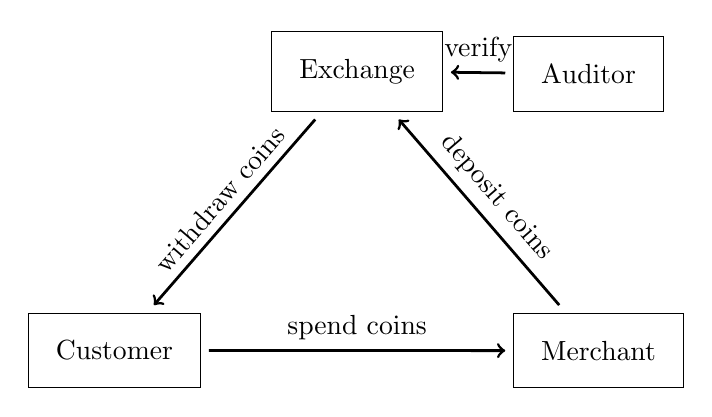
\begin{tikzpicture}
 \tikzstyle{def} = [node distance=3em and 5em, inner sep=1em, outer sep=.3em];
 \node (origin) at (0,0) {};
 \node (exchange) [def,above=of origin,draw]{Exchange};
 \node (customer) [def, draw, below left=of origin] {Customer};
 \node (merchant) [def, draw, below right=of origin] {Merchant};
 \node (auditor) [def, draw, above right=of origin]{Auditor};

 \tikzstyle{C} = [color=black, line width=1pt]

 \draw [<-, C] (customer) -- (exchange) node [midway, above, sloped] (TextNode) {withdraw coins};
 \draw [<-, C] (exchange) -- (merchant) node [midway, above, sloped] (TextNode) {deposit coins};
 \draw [<-, C] (merchant) -- (customer) node [midway, above, sloped] (TextNode) {spend coins};
 \draw [<-, C] (exchange) -- (auditor) node [midway, above, sloped] (TextNode) {verify};

\end{tikzpicture}
\caption{Taler system overview.}
\label{fig:system}
\end{figure}


There are four components of the Taler system (Figure~\ref{fig:system}):

\begin{itemize}
\item
{\em Wallets} are software packages that allow customers to withdraw,
hold, and spend coins.  Wallets also manage the customer's accounts
at the exchange, and keep receipts in a transaction history.  Wallets can be
realized as browser extensions, mobile Apps or even in custom
hardware.

\item
{\em Exchanges}, run by for-profit financial service providers, enable
customers to withdraw anonymous digital coins
and merchants to deposit digital coins, in exchange for
bank money.  Coins are signed by the exchange using
a blind signing scheme \cite{chaum1983blind}.  Thus only
the exchange can issue new coins, but coins can't be traced back
to the customer that withdrew them.
Furthermore, exchanges learn the amounts withdrawn by customers
and deposited by merchants, but they do not learn the relationship
between customers and merchants.  Exchanges perform online detection
of double spending, thus providing merchants instant feedback,
---including digital proofs---in case of misbehaving customers.

\item
{\em Merchants} provide goods or services in exchange for coins held
by customers' wallets.  Merchants deposit these coins at the
exchange for their regular currency value.  Merchants consist of a
{\em frontend} which interacts with the customer's wallet, and a {\em
backend} that interacts with the exchange.  Typical frontends include
Web shops and point-of-sale systems.

\item
{\em Auditors} verify that exchanges operate correctly to limit the risk
that customers and merchants incur by using a particular exchange.
Auditors are typically operated by financial regulatory authorities.
Depending on local legislation, auditors mandate that exchanges
have enough financial reserves before authorizing them to create a given
volume of signed digital coins in order to compensate for potential risks due to
operational failures (such as data loss or theft of private keys) of the exchange.
\end{itemize}

The specific protocol between wallet and merchant depends on the
setting.  For a traditional store, a near field communication (NFC) protocol might be used
between a point-of-sale system and a mobile application.  In this
paper, we focus on Web payments for an online shop.

\begin{figure*}
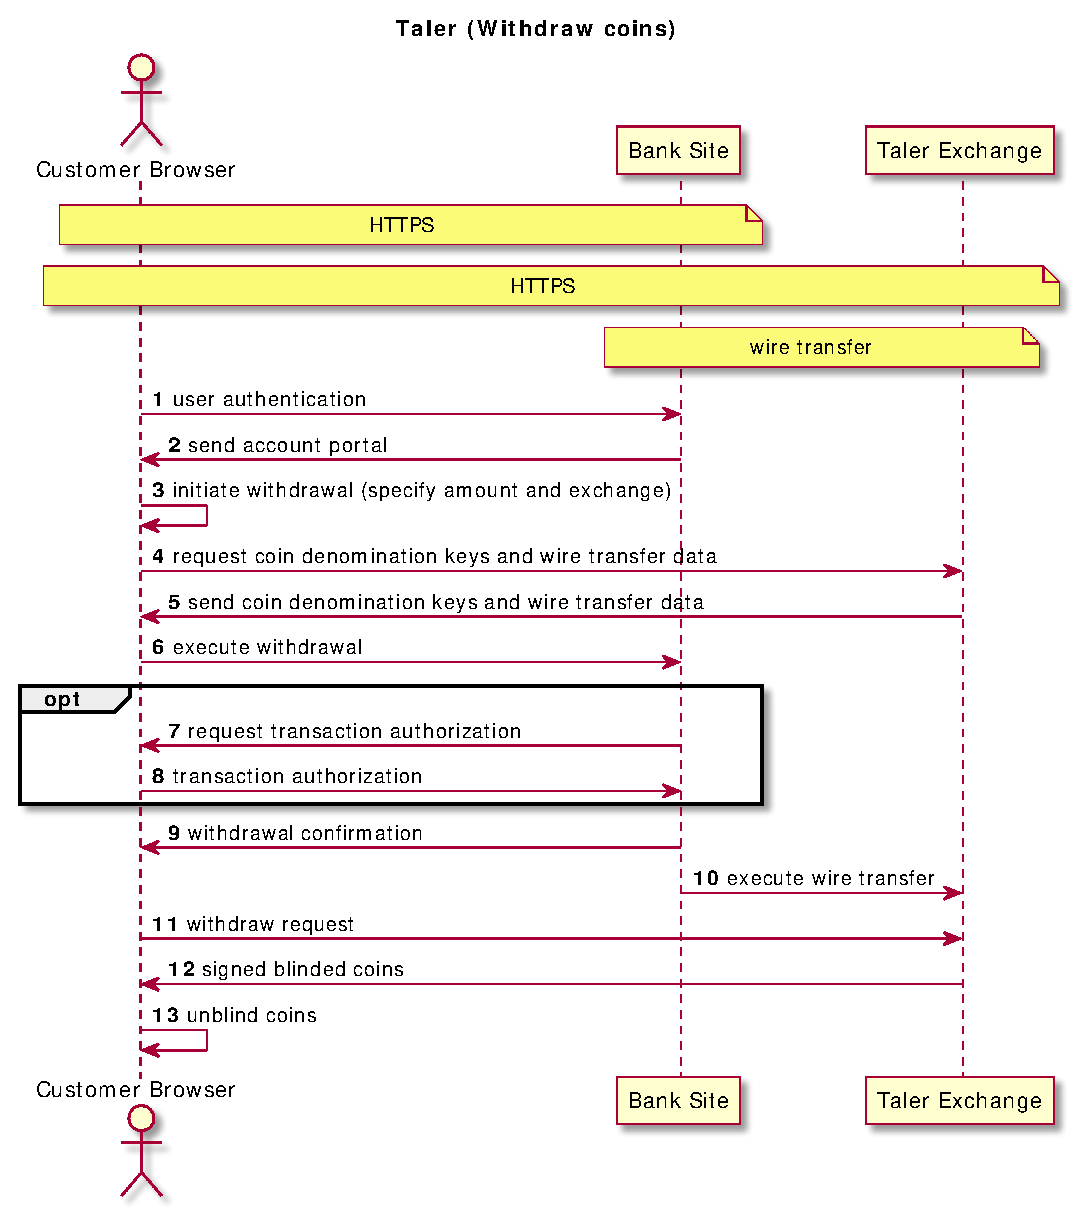
\includegraphics[width=0.9\textwidth]{figs/taler-withdraw.pdf}
\caption{Withdrawing coins with Taler.}
\label{fig:taler-withdraw}
\end{figure*}


% \smallskip
\subsection{Web payment workflow}

We explain how the actors in the Taler system interact by documenting
a typical payment.

Initially, the customer must once install the Taler wallet extension
for their browser.  Naturally, this step may become superfluous if
Taler is integrated tightly with browsers in the future.  Regardless,
installing the extension involves one or two clicks to confirm the
operation once the user was pointed to the correct Web site.
Restarting the browser is not required.

\paragraph{Withdrawing coins}

As with cash, the customer must first withdraw digital coins
(Figure~\ref{fig:taler-withdraw}).  For this, the customer must first
visit the online banking portal of their bank.  Here, the bank will
typically require some form of authentication, the specific method
used depends on the bank (Figure~\ref{subfig:login}).

\begin{figure}
\begin{subfigure}{\linewidth}
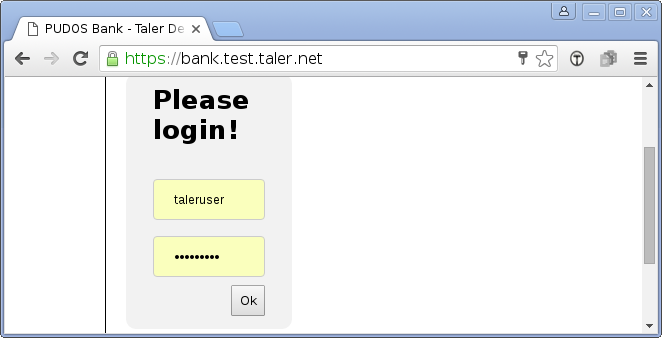
\includegraphics[width=\linewidth]{figs/bank0a.png}
\caption{Bank login. (Simplified for demonstration.)}
\label{subfig:login}
\end{subfigure}
\begin{subfigure}{\linewidth}
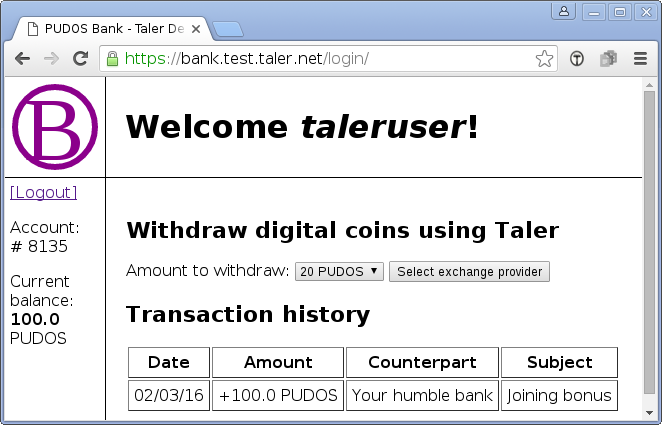
\includegraphics[width=\linewidth]{figs/bank1a.png}
\caption{Specify amount to withdraw. (Integrated bank support.)}
\label{subfig:withdraw}
\end{subfigure}
\begin{subfigure}{\linewidth}
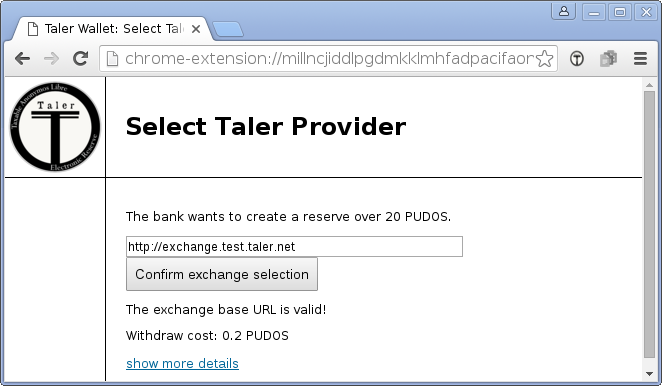
\includegraphics[width=\linewidth]{figs/bank2a.png}
\caption{Select exchange provider. (Generated by wallet.)}
\label{subfig:exchange}
\end{subfigure}
\begin{subfigure}{\linewidth}
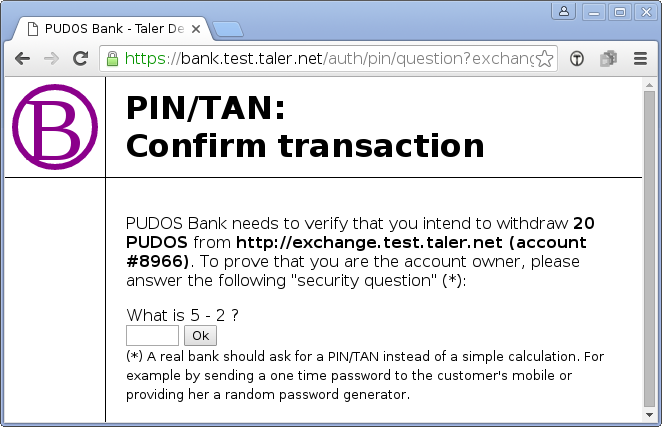
\includegraphics[width=\linewidth]{figs/bank3a.png}
\caption{Confirm transaction with a PIN. (Generated by bank.)}
\label{subfig:pin}
\end{subfigure}
\caption{Required steps in a Taler withdrawal process.}
\label{fig:withdrawal}
\end{figure}


The next step depends on the level of Taler support offered by the bank:
\begin{itemize}
\item If the bank does not offer integration with Taler, the
  customer needs use the menu of the wallet to create a {\em reserve}.
  The wallet will ask which amount in which {\em currency} (i.e. EUR
  or USD) the customer wants to withdraw and allow the customer to
  select an exchange.  Given this information, the wallet will
  instruct the customer to transfer the respective amount to the
  account of the exchange.  The customer will have to enter a
  % FIXME it is not said that this crypto token is the reserve,
  % or, more abstractly, that "identify" this operation
  % CG: I don't think this has to be said.
  54-character reserve key which includes 256 bits of entropy and an
  8-bit checksum into the transfer subject.  Naturally, this is
  exactly the kind of interaction we would like to avoid for
  usability.
\item Hence, if the bank properly integrates with Taler, the
  customer has a form in the online banking portal where they can specify
  an amount to withdraw (Figure~\ref{subfig:withdraw}).
  The bank then triggers an interaction with
  the wallet to allow the customer to select an exchange
  (Figure~\ref{subfig:exchange}).  Afterwards,
  the wallet instructs the bank about the details of the wire
  transfer.  The bank asks the customer to authorize the transfer, and
  finally confirms to the wallet that the transfer has been
  successfully initiated.
\end{itemize}

In either case, the wallet can then withdraw the coins from the
exchange, and does so in the background without further interaction
with the customer.

In principle, the exchange can be directly operated by the bank, in
which case the step where the customer selects an exchange may be
skipped by default.  However, we generally assume that the exchange is
a separate entity, as this yields the largest anonymity set for
customers and may help create a competitive market.

\paragraph{Spending coins}
% \tinyskip

\begin{figure*}
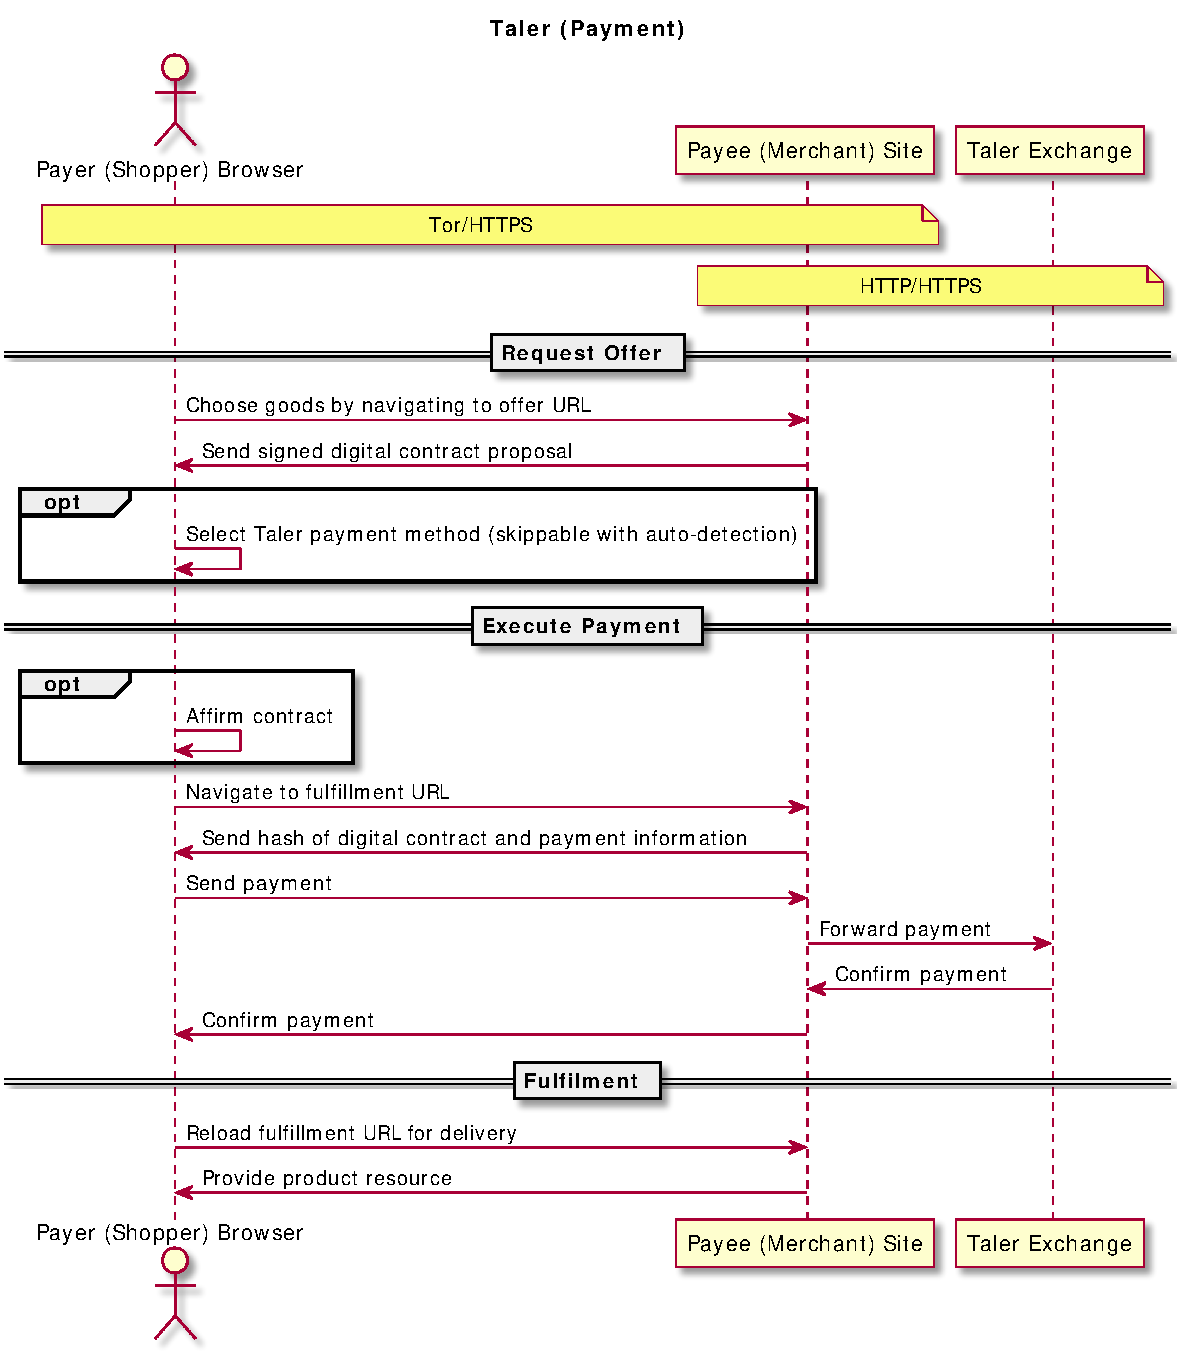
\includegraphics[width=0.9\textwidth]{figs/taler-pay.pdf}
\caption{Payment processing with Taler.}
\label{fig:taler-pay}
\end{figure*}

\begin{figure}[b!]
\begin{subfigure}[H]{0.5\textwidth}
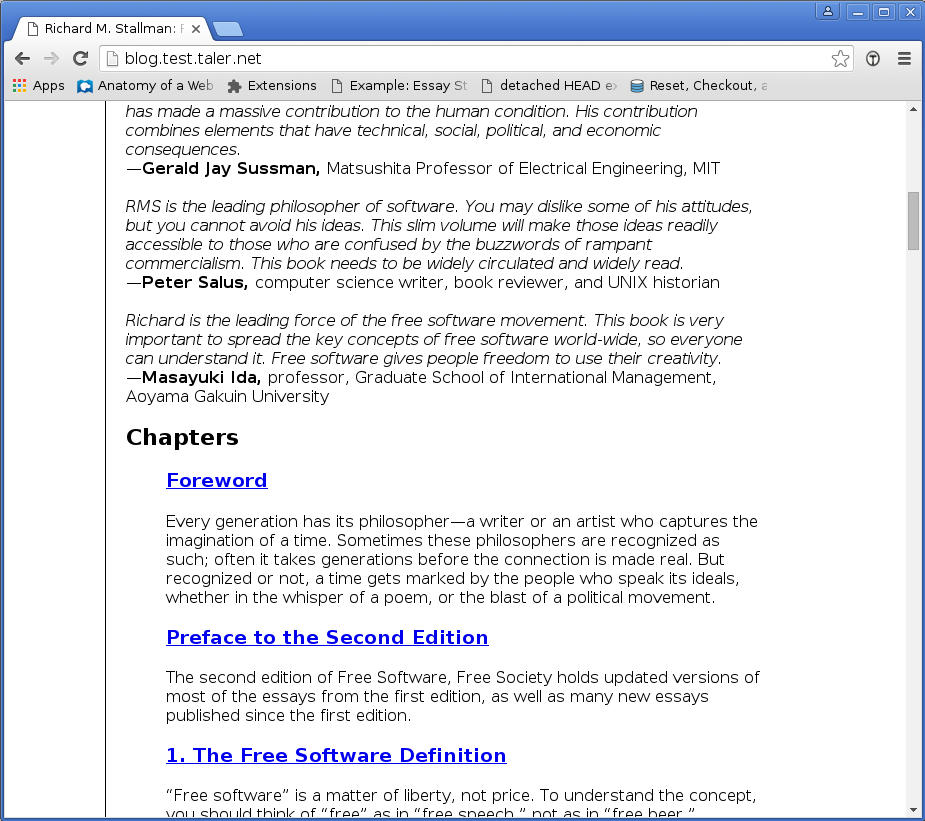
\includegraphics[width=\textwidth]{figs/cart.png}
\caption{Select article. (Generated by Web shop.)}
\label{subfig:cart}
\end{subfigure}
\begin{subfigure}{0.5\textwidth}
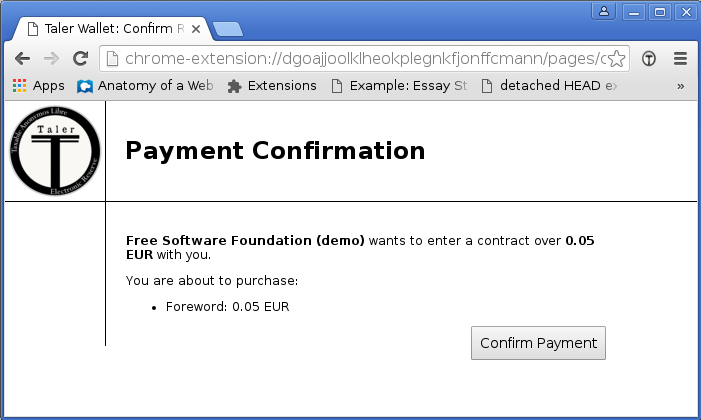
\includegraphics[width=\textwidth]{figs/pay.png}
\caption{Confirm payment. (Generated by Taler wallet.)}
\label{subfig:payment}
\end{subfigure}
\begin{subfigure}{0.5\textwidth}
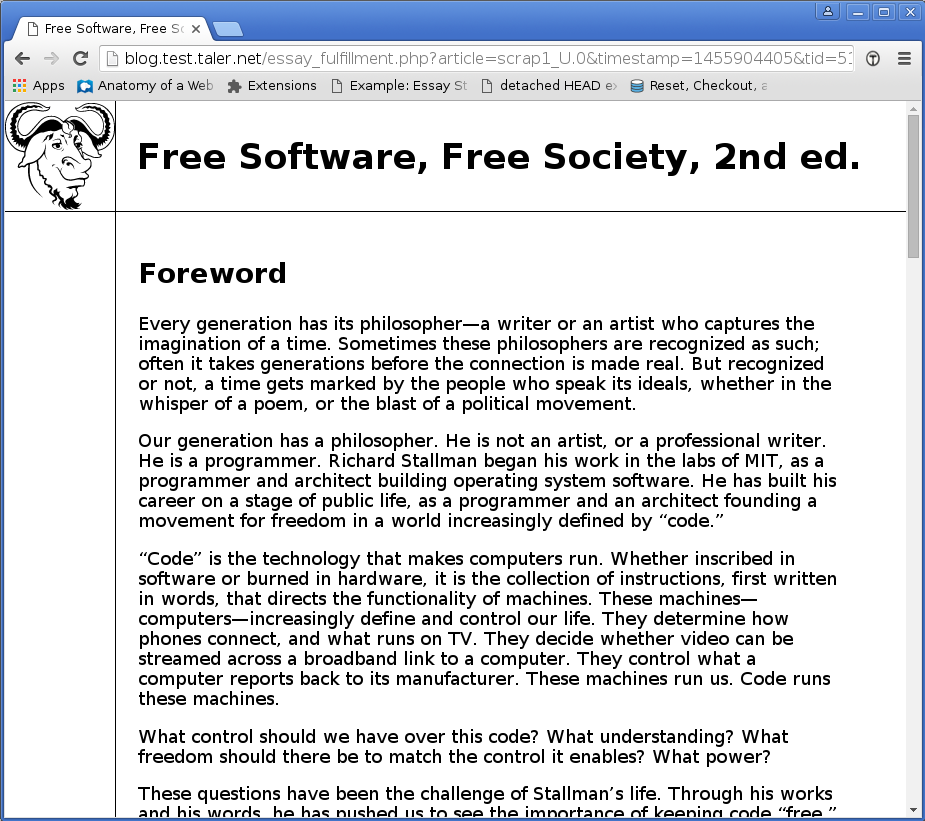
\includegraphics[width=\textwidth]{figs/fulfillment.png}
\caption{Receive article. (Generated by Web shop.)}
\label{subfig:fulfillment}
\end{subfigure}
\caption{Required steps in a Taler checkout process.}
\label{fig:shopping}
\end{figure}


At a later point in time, the customer can spend their coins by
visiting a merchant that accepts digital coins in the respective
currency issued by the respective exchange
(Figure~\ref{fig:taler-pay}).  Merchants are generally configured to
either accept a specific exchange, or to accept all the exchanges
audited by a particular auditor.  Merchants can also set a ceiling for
the maximum amount of transaction fees they are willing to cover.
Usually these details should not matter for the customer, as we expect
most merchants to allow most accredited exchange providers, and for
exchanges to operate with transaction fees acceptable to most
merchants.  If transaction fees are higher than what is covered by the
merchant, the customer may choose to cover them.

As with traditional Web transactions, the customer first selects which
items they wish to buy.  This can involve building a traditional
shopping cart, or simply clicking on a particular link for the
respective article (Figure~\ref{subfig:cart}).  As with card payments,
the Web shop may then allow the customer to select a payment method,
including Taler.  Taler also allows the Web shop to detect
the presence of a Taler wallet (Figure~\ref{listing:presence}), so
that this step may be skipped (as it is in Figure~\ref{fig:shopping}).
If Taler was detected or selected, the Web shop sends a digitally
signed {\em contract proposal} to the wallet extension
(Figure~\ref{listing:contract}).  The wallet then presents the
contract to the user.  The format of the contract is in an extensible
JSON-based format defined by Taler and not HTML, as the
rendering of the contract is done by the wallet to ensure correct
visual representation.  In the case that transaction fees need to be
covered by the customer, these are shown together with the rest of the
proposed contract.

If the customer approves the contract by clicking the ``Confirm
Payment'' button (Figure~\ref{subfig:payment}), their wallet signs the
contract with enough coins to cover the contract's cost, stores all of
the information in its local database, and redirects the browser to a
{\em fulfillment} URL provided by the merchant
(Figure~\ref{subfig:fulfillment}).
% FIXME: technically this is not entirely true, if you
% allow CORS ...
The wallet cannot directly send
the payment to the merchant, as the page showing the contract is
provided as a background page controlled by the Web Extension\footnote{\url{https://developer.chrome.com/extensions}} and thus
submitting coins from the background would not use the HTTP-context
that the Web shop's page requires for session management.

% FIXME: can we do better with the description?
Instead, the server-side of the fulfillment page usually first detects
that the contract has not yet been paid by checking the merchant's
local database and the HTTP session state.  {\bf (A)} If the state
indicates that this customer did not yet pay, the merchant generates a
page that shows the customer an indication that the payment is being
processed, and tries to interact with the wallet, requesting payment.
If the wallet is not detected after a few milliseconds, the page
transitions to the card payment process.  If the wallet is present,
the page requests payment from the wallet.  The wallet then determines
that the customer already confirmed the payment and immediately
transfers the coins to the JavaScript logic of the fulfillment page.
The fulfillment page then transfers the coins to the merchant, usually
using an asynchronous HTTP POST request.  The request is controlled by
the merchant's JavaScript and not by the wallet. This ensures that the
merchant is in full control of the communication between the
merchant's server and the client-side scripts interacting with the
merchant's server.  The interactions with the wallet are thus purely
local interactions within the browser.  Upon receipt of the payment
information, the merchant confirms the payment with the exchange,
marks the payment as received, and notifies the JavaScript on the
client side of the result.

\begin{itemize}
\item If the payment fails on the network, the request is typically
 retried.  How often the client retries automatically before informing
 the user of the network issue is up to the merchant.  If the network
 % FIXME this (above) could be ambiguous because the network failure
 % can happen between the wallet and the merchant without the merchant
 % getting any (failing) request, so the merchant cannot count how much
 % times a payment has failed.
 % CG: Well, the merchant can do that counting *client-side*. The retries
 % will be controlled by the JS on the client side, which is provided
 % by the merchant initially.
 failure persists and is between customer and merchant, the wallet
 will try to recover control over the coins at the exchange by
 effectively spending the coins first using Taler's special
 % FIXME(dold):  Do we properly introduce/discuss refreshing before?
 ``refresh'' protocol.  In this case, later deposits by the merchant
 will simply fail.  If the merchant already succeeded with the payment
 before the network failure, the customer can either retry the
 operation later via the transaction history, or demand a refund (see
 below).  Handling these errors does not require the customer to give
 up his privacy.
\item If the payment fails due to the exchange
 claiming that the request was invalid, the diagnostics created by the
 exchange are passed to the wallet for inspection.  The wallet then
 decides whether the exchange was correct, and can then inform the
 user about a fraudulent or buggy exchange.  At this time, it allows
 the user to export the relevant cryptographic data to be used in
 court.  If the exchange's proofs were correct and coins were
 double-spent, the wallet informs the user that its database must have
 % FIXME what about giving an example of an out-of-date DB?  Put in
 % this way, it appears that Taler has viable ways to fail. In other
 % words, that it's normal to get such a failure. Instead, that failure
 % can occur due to coins not spent for *years* (or some other corner case),
 % that saves Taler from being "blamed"
 been out-of-date, updates the database and allows the user to retry
 the transaction.
\item If the payment succeeded, the JavaScript on the
 client side triggers effectively a ``reload'' of the fulfillment
 page, triggering case (B) detailed below.
\end{itemize}

{\bf (B)} Upon subsequent visits, the server detects that the payment
has already been processed and directly generates a fulfillment page
either confirming the payment, or---in the case of payments for a
digital article---transmits the digital artifact to the client.

\paragraph{Bookmarks and deep links}

This particular architecture also enables smooth use of the payment
URIs on the contemporary Web.  In particular, we need to consider the
possibility that a user may bookmark the fulfillment page, or forward
a link to the fulfillment page to another user.

The given design supports {\em bookmarking}. If the merchant's
session management is still tracking the user when he returns via the
bookmark, the page generation detects that the user has already paid
and serves the final fulfillment page.  If the session has been lost,
the merchant will generate a fulfillment page asking for payment.  In
this case, the wallet will detect that it has already paid this
contract via a unique identifier in the contract, and will
automatically re-play the payment.  The merchant confirms that this
customer already paid, and generates the final fullfilment page that the
user has previously payed for (and seen).  All this still appears as
instantaneous to the user as it merely adds a few extra network round trips.

In contrast, if the customer sends a link to the fulfillment page to
another user, thereby possibly sharing a {\em deep link} into the
merchant's shop, the other customer's wallet will fail to find an
existing payment.  Consequently, the fulfillment page will not receive
the payment details and instead provide the user with the proposed
contract which contains a description of the item previously bought by
the other user. The recipient of the link can then decide to also
purchase the item.

The design, in particular POSTing the coins asyn\-chro\-nous\-ly from
JavaScript, also ensures that the user can freely navigate with
the back and forward buttons.  As all requests from all HTTP(S)
URIs ever seen by the user in the browser are fetched via HTTP
GET, they can be bookmarked, shared and safely reloaded.  For
caching, the merchant needs to ensure that the fulfillment
page generated in case (A) is not cached by the browser,
and in case (B) is not cached in the network.

As an aside, there are actually several distinct roles comprising the
merchant: shopping pages end their role by proposing a contract, while
a fulfillment page begins its life processing a contract.  It is thus
possible for these components being managed by separate parties. The
control of the fulfillment page over the transmission of the payment
information minimizes the need for exceptions to handle cross-origin
resource sharing.~\cite{rfc6454,cors}

% FIXME: for the above: add figures with code samples!
% \smallskip

\paragraph{Giving change and refunds} % FIXME: maybe leave out change entirely?

An important technical difference between Taler and previous
transaction systems based on blind signing is that Taler is able to
provide unlinkable change and refunds.  From the user's point of view,
obtaining change is automatic and handled by the wallet, i.e. if the
user has a single coin worth \EUR{5} and wants to spend \EUR{2}, the
wallet may request three \EUR{1} coins in change --- critically, this
is completely hidden from the user. In fact, the graphical user
interface does not offer a way to inspect the denominations of the
various coins in the wallet, it only shows the total amount available
in each denomination.  Expanding the views to show details may show
the exchange providers and fee structure, but not the cryptographic
coins.  Consequently, the major cryptographic advances of Taler are
invisible to the user.

Taler's technology also allows merchants to give refunds to
customers. For this, the merchant merely has to send a signed
message to the exchange confirming the refund, and notify the
customer's wallet that the respective transaction was refunded.
This can even be done with anonymous customers, as refunds are
given as additional change to the owner of the coins that were
originally spent to pay for the refunded transaction.

Taler's protocol ensures unlinkability for both changes and refunds,
thus assuring that the user has key conveniences of other payment
systems, while maintaining the security standard of an anonymous
payment system.

% Alternative version:
%An important technical difference between Taler and previous
%transaction systems based on blind signing is that in Taler coins
%consist of a public-private key pair with the blind signature on the
%public key, so that coins themselves can be used to anonymously sign
%the purchase contract.
%
%An important technical difference between Taler and previous
%transaction systems based on blind signing is that Taler coins
%consist of a public-private key pair with the blind signature on the
%public key, so that coins themselves can be used to anonymously sign
%the purchase contract.
%
%In general, these coins exceed the cost of the contract, so the wallet
%may specify that only a fraction of a coin be spent, leaving some
%residual value on the partially spent coin as ``change''.
%
%As the merchant received only a signature of the coin, not private
%or symmetric key material, merchants can refund anonymous coins by
%asking the mint to restore a part of the coin's original value,
%and notifying the customer's wallet to refresh the coin.
%
%Spending Taler coins reveals nothing about a customer per se.
%Yet, any coins that hold value after being involved in a purchase or
%a refund operation cannot be considered anonymous anymore because a
%merchant, and possibly the exchange, has now seen them and could
%link them that previous transaction.  At best, these tainted coins
%are only pseudononymous, similar to Bitcoin accounts.
%
%To maintain anonymity, a Taler wallet automatically performs a
%{\em refresh} operation with the mint API to both replace tainted
%coins with new freshly anonymized coins and to exchange old coins
%before their denomination's expiration date.  We view refreshing
%partially spent coins as analogous to giving change in cash
%transactions, but refreshing refunded coins allows Taler merchants
%to refund anonymous customers.  Cash transactions have these options,
%but credit cards require customer identification for both operations.
% Is this true?
% no comment around randomizing the serial numbers on bills


\subsection{NFC payments}

We have so far focused on how Taler would be used for Web payments;
however, Taler can also be naturally used over other protocols, such
as near field communication (NFC).  Here, the user would hold his
NFC-enabled device running a wallet application near an NFC terminal
to obtain the contract and confirm the payment on his device, which
would then transfer the coins and obtain a receipt.  An NFC
application would be less restricted in its interaction with the
point-of-sale system compared to a browser extension; thus, running
Taler over NFC is largely a simplification.

Specifically, there are no significant new concerns arising from an
NFC device possibly losing contact with a point-of-sale system.
Already for Web payments, Taler employs only idempotent operations to
ensure coins are never lost and that transactions adequately persist
even in the case of network or endpoint failures.  As a result, the
NFC system can simply use the same transaction models to replay
transmissions once contact with the point-of-sale system is
reestablished.


\subsection{Peer-to-peer payments}

Peer-to-peer payments are possible with Taler as well; however,
we need to distinguish two types of peer-to-peer payments.

First, there is the {\em sharing} of coins among entities that
mutually trust each other, for example within a family.  Here, all the
users have to do is to export and import electronic coins over a
secure channel, such as encrypted e-mail or via NFC.  For NFC, the
situation is pretty trivial, while secure communication over the
Internet is likely to remain a significant usability challenge.  We
note that sharing coins by copying the respective private keys across
devices is not taxable: the exchange is not involved, no contracts are
signed, and no records for taxation are created.  However, the
involved entities must trust each other, as after copying a private
key both parties could spend the coins, but only the first transaction
will succeed.  Given this crucial limitation
inherent in sharing keys, we consider it ethically acceptable that
sharing is not taxable.

Second, there is the {\em transactional} mutually exclusive transfer
of ownership.  This requires the receiving party to have a {\em
reserve} with an exchange, and the exchanges would have to support
wire transfers among them.  If taxability is desired, the {\em
reserve} would still need to be tied to a particular citizen's
identity for tax purposes, and thus require similar identification
protocols as commonly used for establishing a bank account. Thus, in
terms of institutions, one would expect this setup to be offered most
easily by traditional banks.  In terms of usability, transactional
transfers are just as easy as sharing when performed over NFC, but
more user friendly when performed over the Internet as they do not
require a secure communication channel: the Taler protocol is by
design still safe to use even if the communication is made over an
unencrypted channel. Only the authenticity of the proposed contract
needs to be assured.


\subsection{Usability for merchants}

Payment system security and usability is not primarily a concern for
customers, but also for merchants.  For consumers, existing schemes
may be inconvenient and not provide privacy, but remembering to
protect a physical token (i.e. the card) and to guard a secret
(i.e. the PIN) is relatively straightforward.  In contrast, merchants
are expected to ``securely'' handle sensitive customer payment data on
networked computing devices.  However, securing computer systems---and
especially payment systems that represent substantial value---is a
hard challenge, as evidenced by large-scale break-ins with millions of
consumer card records being illicitly copied.~\cite{target}

Thus, we cannot ignore the usability at the merchant site when trying
to understand the usability of a payment system, especially as for
deployment we will have to convince millions of merchants that the
Taler system is advantageous.  The high-level cryptographic design
already provides the first major advantage, as merchants do never
receive sensitive payment-related customer information.  Thus, they do
% FIXME as *it* is ?
% CG: both are OK in English, ``it'' can be omitted here.
not have to be subjected to costly audits or certified hardware, as is
commonly the case for processing card payments.~\cite{pcidss} In fact,
the exchange does not need to have a formal business relationship with
the shop at all.  According to our design, the exchange's contract
with the state regulator or auditor and the customers ought to state
that it must honor all (legal and valid) deposits it receives.  Hence,
a merchant supplying a valid deposit request should be able to enforce
this in court without a prior business agreement with the exchange.
This dramatically simplifies setting up a shop, to the point that the
respective software only needs to be provided with the merchant's wire
transfer routing information to become operational.

Figure~\ref{listing:presence} shows how easy it is for a Web shop to
detect the presence of a Taler wallet.  This leaves a few cryptographic
operations, such as signing a contract and verifying the customer's and
the exchange's signatures, storing transaction data as well as matching
sales with incoming wire transfers from the exchange.  Taler simplifies this
for merchants by providing a generic payment processing {\em backend} for
the Web shops.

\begin{figure*}[h!]
\begin{center}
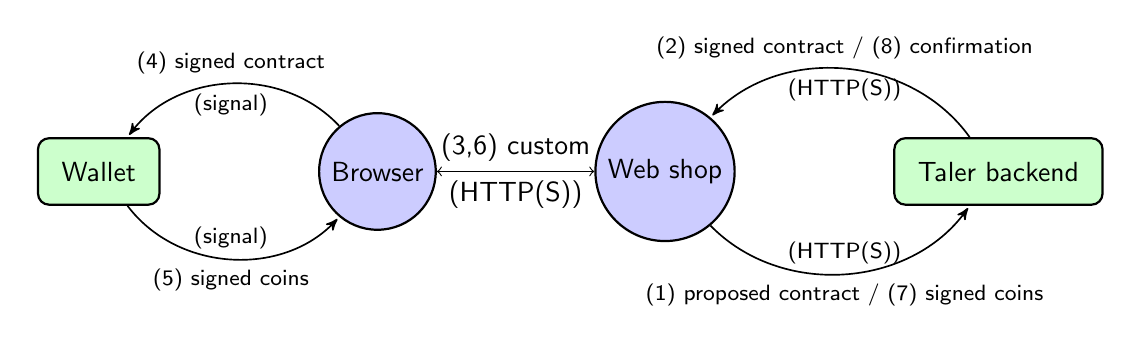
\begin{tikzpicture}[
  font=\sffamily,
  every matrix/.style={ampersand replacement=\&,column sep=2cm,row sep=2cm},
  source/.style={draw,thick,rounded corners,fill=green!20,inner sep=.3cm},
  process/.style={draw,thick,circle,fill=blue!20},
  sink/.style={source,fill=green!20},
  datastore/.style={draw,very thick,shape=datastore,inner sep=.3cm},
  dots/.style={gray,scale=2},
  to/.style={->,>=stealth',shorten >=1pt,semithick,font=\sffamily\footnotesize},
  every node/.style={align=center}]

  % Position the nodes using a matrix layout
  \matrix{
    \node[source] (wallet) {Wallet};
      \& \node[process] (browser) {Browser};
      \& \node[process] (shop) {Web shop};
      \& \node[sink] (backend) {Taler backend}; \\
  };

  % Draw the arrows between the nodes and label them.
  \draw[to] (browser) to[bend right=50] node[midway,above] {(4) signed contract}
      node[midway,below] {(signal)} (wallet);
  \draw[to] (wallet) to[bend right=50] node[midway,above] {(signal)}
      node[midway,below] {(5) signed coins} (browser);
  \draw[<->] (browser) -- node[midway,above] {(3,6) custom}
      node[midway,below] {(HTTP(S))} (shop);
  \draw[to] (shop) to[bend right=50] node[midway,above] {(HTTP(S))}
      node[midway,below] {(1) proposed contract / (7) signed coins} (backend);
  \draw[to] (backend) to[bend right=50] node[midway,above] {(2) signed contract / (8) confirmation}
      node[midway,below] {(HTTP(S))} (shop);
\end{tikzpicture}
\end{center}
 \caption{Both the customer's client and the merchant's server
          execute sensitive cryptographic operations in a
          secured background/backend that is protected against direct access.
          Interactions with the Taler exchange from the wallet background
          to withdraw coins and the Taler backend (Figure~\ref{fig:system})
          to deposit coins are not shown.
          Existing system security mechanisms
          are used to isolate the cryptographic components (boxes) from
          the complex rendering logic (circles), hence the communication
          is restricted to JavaScript signals or HTTP(S) respectively.}
 \label{fig:frobearch}
\end{figure*}

Figure~\ref{fig:frobearch} shows how the secure payment components
interact with the existing Web shop logic.  First, the Web shop
frontend is responsible for constructing the shopping cart.  For this,
the shop frontend generates the usual Web pages which are shown to the
user's browser client frontend.  Once the order has been constructed,
the shop frontend gives a {\em proposed contract} in JSON format to the
payment backend, which signs it and returns it to the frontend.  The frontend
then transfers the signed contract over the network, and passes it to the
wallet (sample code for this is in Figure~\ref{listing:contract}).
Here, the wallet operates from a secure {\em background} on the client side,
which allows the user to securely accept the payment, and to perform
the cryptographic operations in a context that is protected from the
Web shop. In particular, it is secure against a merchant that
generates a page that looks like the payment page from the wallet
(Figure~\ref{subfig:payment}), as such a page would still not have
access to the private keys of the coins that are in the wallet.  If
the user accepts, the resulting signed coins are transferred from the
client to the server, again by a protocol that the merchant can
customize to fit the existing infrastructure.

Instead of adding any cryptographic logic to the merchant frontend,
the generic Taler merchant backend allows the implementor to delegate
handling of the coins to the payment backend, which validates the
coins, deposits them at the exchange, and finally validates and
persists the receipt from the exchange.  The merchant backend then
communicates the result of the transaction to the front\-end, which is
then responsible for executing the business logic to fulfill the
order.  As a result of this setup, the cryptographic details of the
Taler protocol do not have to be re-implemented by each merchant.
Instead, existing Web shops implemented in a multitude of programming
languages can rather trivially add support for Taler by {\bf (0)}
detecting in the browser that Taler is available, {\bf (1)} upon
request, generating a contract in JSON based on the shopping cart,
{\bf (2)} allowing the backend to sign the contract before sending it
to the client, {\bf (7)} passing coins received in payment for a
contract to the backend and {\bf (8)} executing fulfillment business
logic if the backend confirms the validity of the payment.

To setup a Taler backend, the merchant only needs to let it know his wire
transfer routing details, such as an IBAN number.  Ideally, the
merchant might also want to obtain a certificate for the public key
generated by the backend for improved authentication.  Otherwise, the
customer's authentication of the Web shop simply continues to rely
upon HTTPS/X.509.


\section{Discussion}

We will now discuss how customer's may experience relevant operational
risks and failure modes of Taler, and relate them to failure modes
in existing systems.

% \smallskip
\subsection{Security risks}

In Taler, customers incur the risk of wallet loss or theft.  We
believe customers can manage this risk effectively because they manage
similar risks of losing cash in a physical wallet.  Unlike physical
wallets, Taler's wallet could be backed up to secure against loss of a
device.

Taler's contracts do provide a degree of protection for customers
because they are signed by the merchant and retained by the wallet:
while they mirror the paper receipts that customers may receive in
physical stores, Taler's cryptographically signed contracts ought to
carry more weight in courts than typical paper receipts.

Point-of-sale systems providing printed receipts have been compromised
in the past by merchants to embezzle sales
taxes.~\cite{munichicecream} With Taler, the merchant still generates
a receipt for the customer; however, the record for the tax
authorities ultimately is anchored with the exchange's wire transfer
to the merchant.  Using the subject of the wire transfer, the state
can trace the payments and request the merchant to provide
cryptographically matching contracts.  Thus, this type of tax
fraud is no longer possible, which is why we call Taler {\em
taxable}.  The mere threat of the state sometimes tracing transactions
and contracts back to the merchant also makes Taler unsuitable for
illegal activities.

The exchange operator is obviously crucial for risk management in
Taler, as the exchange operator holds the customer's funds in a
reserve in escrow until the respective deposit request arrives\footnote{As
previously said, this {\it deposit request} is aimed to translate {\it coins}
into real money and it's accomplished by a merchant after successfully
receiving coins by a wallet. In other words, it is the way merchants get
real money on their bank accounts}. To ensure that the exchange operator
does not embezzle these funds, Taler expects exchange operators to be
regularly audited by an independent auditor\footnote{Auditors are typically
run by financial regulatory bodies of states}.  The auditor can then verify that the incoming and outgoing
transactions and the current balance of the exchange match the logs
with the cryptographically secured transaction records.


% \smallskip
\subsection{Failure modes}

There are several failure modes the user of a Taler wallet may
encounter:

\begin{itemize}
\item
As Taler supports multiple exchanges, there is a chance that a
merchant might not support any exchange where the customer withdrew
coins from.  We mitigate this problem by allowing merchants to
support all exchanges audited by a particular auditor.  We believe
this a reasonable approach, because auditors and merchants must
operate with a particular legal and financial framework anyways.  We
note that a similar failure mode exists with credit cards, where not
all merchants accept all issuers, especially internationally.

\item
Restoring the Taler wallet state from previous backups, or copying the
wallet state to a new machine, may cause honest users to attempt to
double spend coins, as the wallet does not know when coins are spent
between backup and recovery.  In this case, the exchange provides
cryptographic proof that the coins were previously spent, so the
wallet can verify that the exchange and merchant are behaving honestly.

% FIXME FIXME: the following paragraph seems to describe a scenario where the
% wallet lost coins due to a restore from backup and then ask for refresh
% of lost coins: but how does the wallet know lost coins' public keys?
% CG: I don't understand the problem.
%
% Also in this paragraph: how can a payment end in-flight due to insufficient
% funds? If the payment has been started by the wallet, then no 'insufficient
% funds' may occur, otherwise the wallet would not have started the payment.
%
% CG: Yes, as I explain if the Wallet isn't aware that some coins were
% already spent (I make a backup, spend coins, restore backup, try to
% spend again), then this may happen.
%
% A way to fix that could be to better define 'internal invariants' ..
%
% CG: The internal invariant is exactly the one you fell upon:
% That the wallet knows which coins have been spent!
\item
There could be insufficient funds in the Taler wallet when making a
payment.  Usually the wallet can trivially check this before beginning
a transaction, but when double-spending is detected this may also
happen after the wallet already initiated the payment. This would
usually only happen if the wallet is unaware of a backup operation
voiding its internal invariants.  If a payment fails in-flight due to
insufficient funds, the wallet can use Taler's refresh protocol to
obtain a refund for those coins that were not actually double-spent,
and then explain the user that the balance was inaccurate due to
inconsistencies from recovery, and overall insufficient for payment.
For the user, this failure mode appears equivalent to an insufficient
balance or credit line when paying with cards.
\end{itemize}

\subsection{Comparison}

The different payment systems discussed make use of different security
technologies, which has an impact on their usability and the
assurances they can provide.  Except for Bitcoin, all payment systems
described involve an authentication step.
% FIXME alternative for the following sentence:
% With Taler, the authentication is implicit when withdrawing, since
% the user has to login into his bank's Web portal in the first place,
% and no further authentication is required during the whole payment
% experience.
% CG: Not exactly, as the authentication to the bank is still
% a very explicit authentication step. It's just more natural.
With Taler, the authentication itself is straightforward, as the customer is
at the time visiting the Web portal of the bank, and the authentication is
with the bank (Figure~\ref{fig:taler-withdraw}).  With PayPal, the
shop redirects the customer to the PayPal portal (step 5 in
Figure~\ref{fig:paypal}) after the user selected PayPal as the payment
method. The customer then provides the proof of payment to the
merchant.  Again, this is reasonably natural.  The 3DS workflow
(Figure~\ref{fig:cc3ds}) has to deal with a multitude of banks and
their different implementations, and not just a single provider.
Hence, the interactions are more complicated as the merchant needs to
additionally perform a lookup in the card scheme directory and verify
availability of the bank (steps 8 to 12).

The key difference between Taler and 3DS or PayPal is that
in Taler, authentication is done ahead of time.
After authenticating once to withdraw digital coins, the customer can
perform many micropayments without having to re-authenticate.  While
this simplifies the process of the individual purchase, it shifts the
mental overhead to an earlier time, and thus requires some planning,
especially given that the digital wallet is likely to only contain a
% FIXME line below: which 'funds'? Coins or real money? (If they are
% coins, recall that the wallet withdraw all the coins from a fresh
% reserve, so there is no 'fraction' of user's available funds; at
% least in the current implementation)
% I originally wrote ``wealth'' or ``net value'', but given that
% most customers are in debt today, that makes little sense, so
% I changed it to ``available funds'', but I meant _all_ the money
% he has.
small fraction of the customer's available funds.  As a result, Taler
improves usability if the customer is able to withdraw funds once to
then facilitate many micropayments, while Taler is likely less usable
if for each transaction the customer first visits the bank to withdraw
funds.  This is deliberate, as Taler can only achieve reasonable
privacy for customers if they do keep a balance in their wallet,
thereby breaking the association between withdrawal and deposit.
% FIXME the sentence above can be in contrast with how the exchange
% actually deposits funds to merchants, that is through 'aggregate
% deposits' that may add unpredictable delays (but that doesn't affect
% this article too much)
% CG: I think mentioning aggregation here would distract.

Bitcoin's payment process (Figure~\ref{fig:bitcoin}) resembles that of
Taler in one interesting point, namely that the wallet is given
details about the contract the user is to enter (steps 7 to 11).
However, in contrast to Taler, here the Bitcoin wallet(s) are expected
to fetch the ``invoice'' from the merchant, while in Taler the browser
provides the Taler wallet with the proposed contract directly.  In
PayPal and 3DS, the user is left without a cryptographically secured
receipt.

Card-based payments (including 3DS) and PayPal also extensively rely
on TLS for security.  The customer is expected to verify that their
connections to the various Web sites are properly authenticated using
X.509, and to know that it is fine to provide their bank account
credentials to the legitimate
\url{verifiedbyvisa.com}.\footnote{The search query
``verifiedbyvisa.com legit'' is so common that, when we entered
``verifiedbyvisa'' into a search engine, it was the suggested
auto-completion.}  However, relying on users understanding their
browser's indications of the security context is inherently
problematic.  Taler addresses this challenge by ensuring that digital
coins are only accessible from fully wallet-generated pages, hence
there is no risk of Web pages mimicking the look of the respective
page, as they would still not obtain access to the digital coins.

Once the payment process nears its completion, merchants need to have
some assurance that the contract is now valid.  In Taler, merchants
obtain a non-repudiable confirmation of the payment.  With 3DS and
PayPal, the confirmation may be disputed later (i.e. in case of
fraud), or accounts may be frozen arbitrarily~\cite{diaspora2011}.
Payments in cash require the merchant to assume the risk of receiving
counterfeit money.
% FIXME what about (for the following sentence): merchants should care
% about maintaining change and depositing the money earned
% CG: No, it's not optional, ``should'' doesn't come into the equation
% here. It's a mandatory business expense.
Furthermore, merchants have the cost maintaining change and depositing
the money earned.  With Bitcoin, there is no definitive time until a
payment can be said to be confirmed (step 19, Figure~\ref{fig:bitcoin}),
leaving merchants in a bit of a tricky situation.

\section{Conclusion}

Customers and merchants should be able to easily adapt their existing
mental models and technical infrastructure to Taler.  In contrast,
Bitcoin's payment models fail to match common expectations, be it in
terms of performance, durability, security, or privacy.  Minimizing
the need to authenticate to pay fundamentally improves usability.

% FIXME (following paragraph): it's never said that the Taler wallet
% keeps any 'receipt' of transaction -- maybe here we want to say 'contract'
% instead of 'receipt'?
% CG: I'd say on the customer side, the signed contract is a receipt.
% That should be intuitive.
We expect that electronic wallets that automatically collect digitally
signed receipts for transactions will become commonplace.  A key
question for the future is thus whether this data collection will be
done on behalf of the citizens and under their control, or on behalf
of the Reich of big data corporations.

We encourage readers to try our prototype for Taler
at \url{https://demo.taler.net/}, and to ponder why the billion dollar
e-commerce industry still relies mostly on TLS for security, given
that usability, security and privacy can clearly {\em all} be improved
simultaneously using a modern payment protocol.

% These APIs are all RESTful in the modern sense because that greatly
% simplify integrating Taler with web shops and browsers.

\section*{Acknowledgements}

This work benefits from the financial support of the Brittany Region
(ARED 9178) and a grant from the Renewable Freedom Foundation.

\bibliographystyle{abbrv}
\bibliography{ui,btc,taler,rfc}

\appendix

\begin{figure*}
\begin{center}
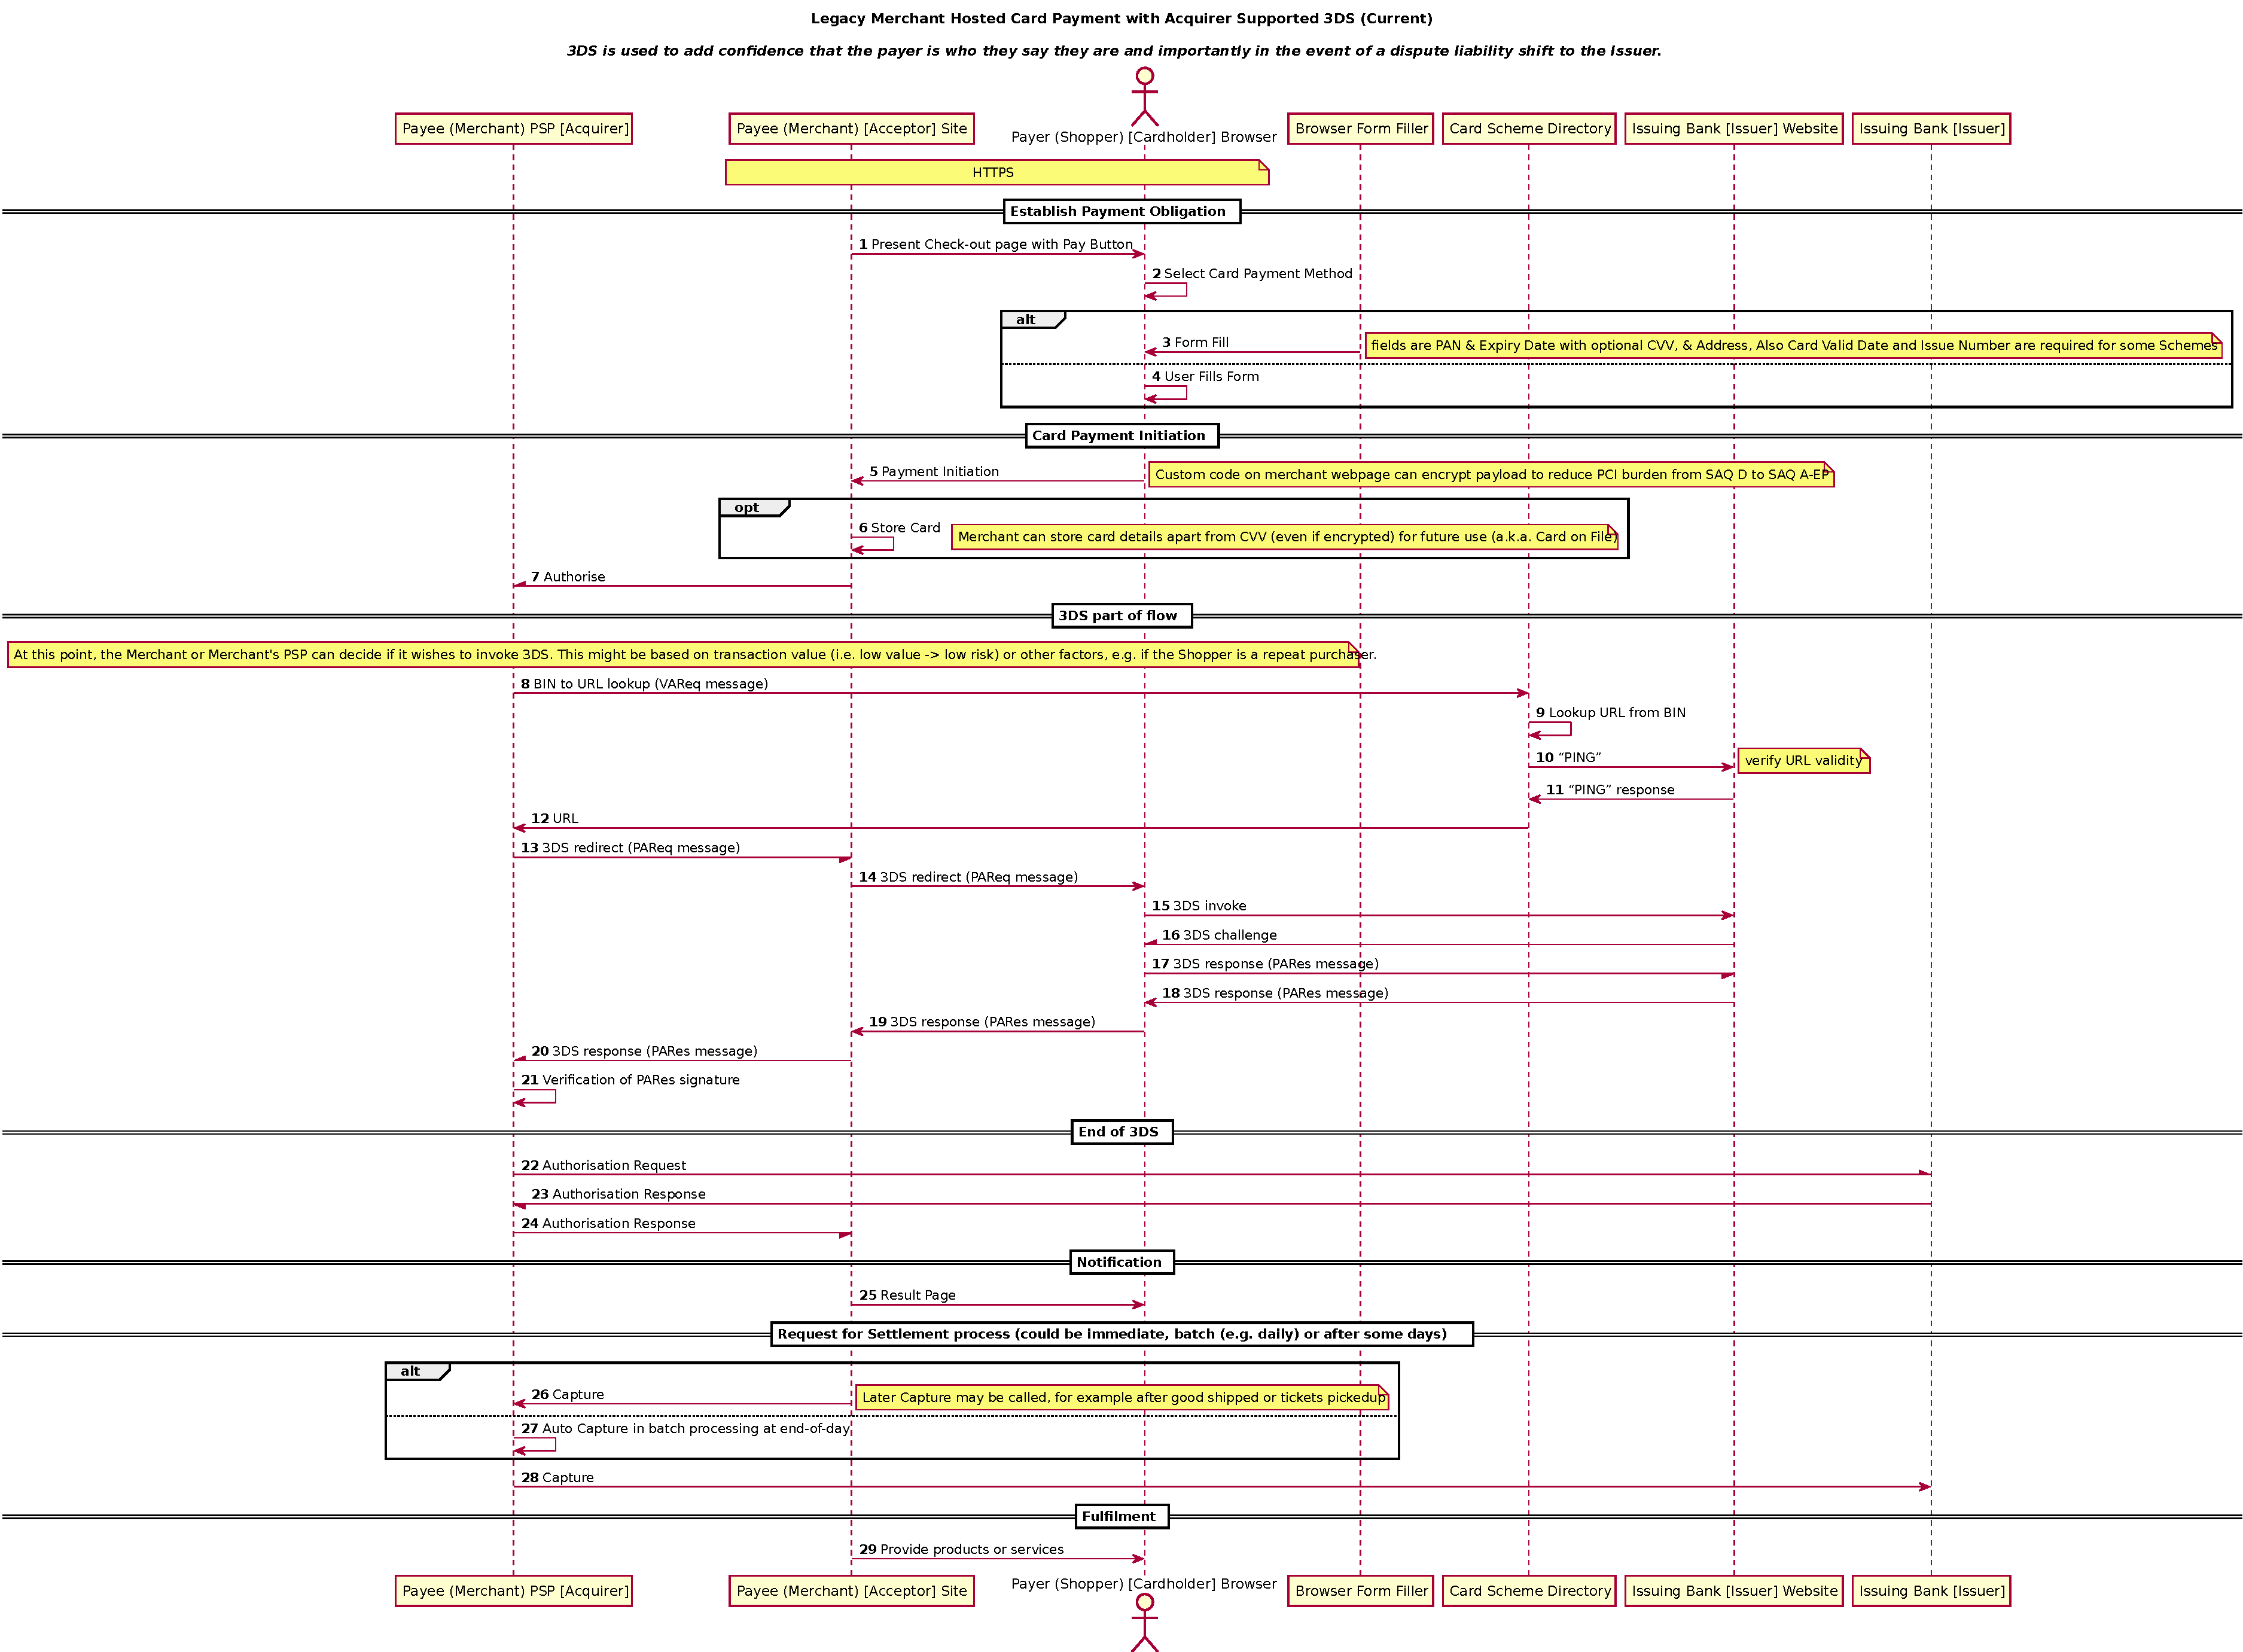
\includegraphics[width=0.95\textwidth]{figs/cc3ds.pdf}
\end{center}
\caption{Card payment processing with 3DS. (From: W3c Web Payments IG.)}
\label{fig:cc3ds}
\end{figure*}



\begin{figure*}
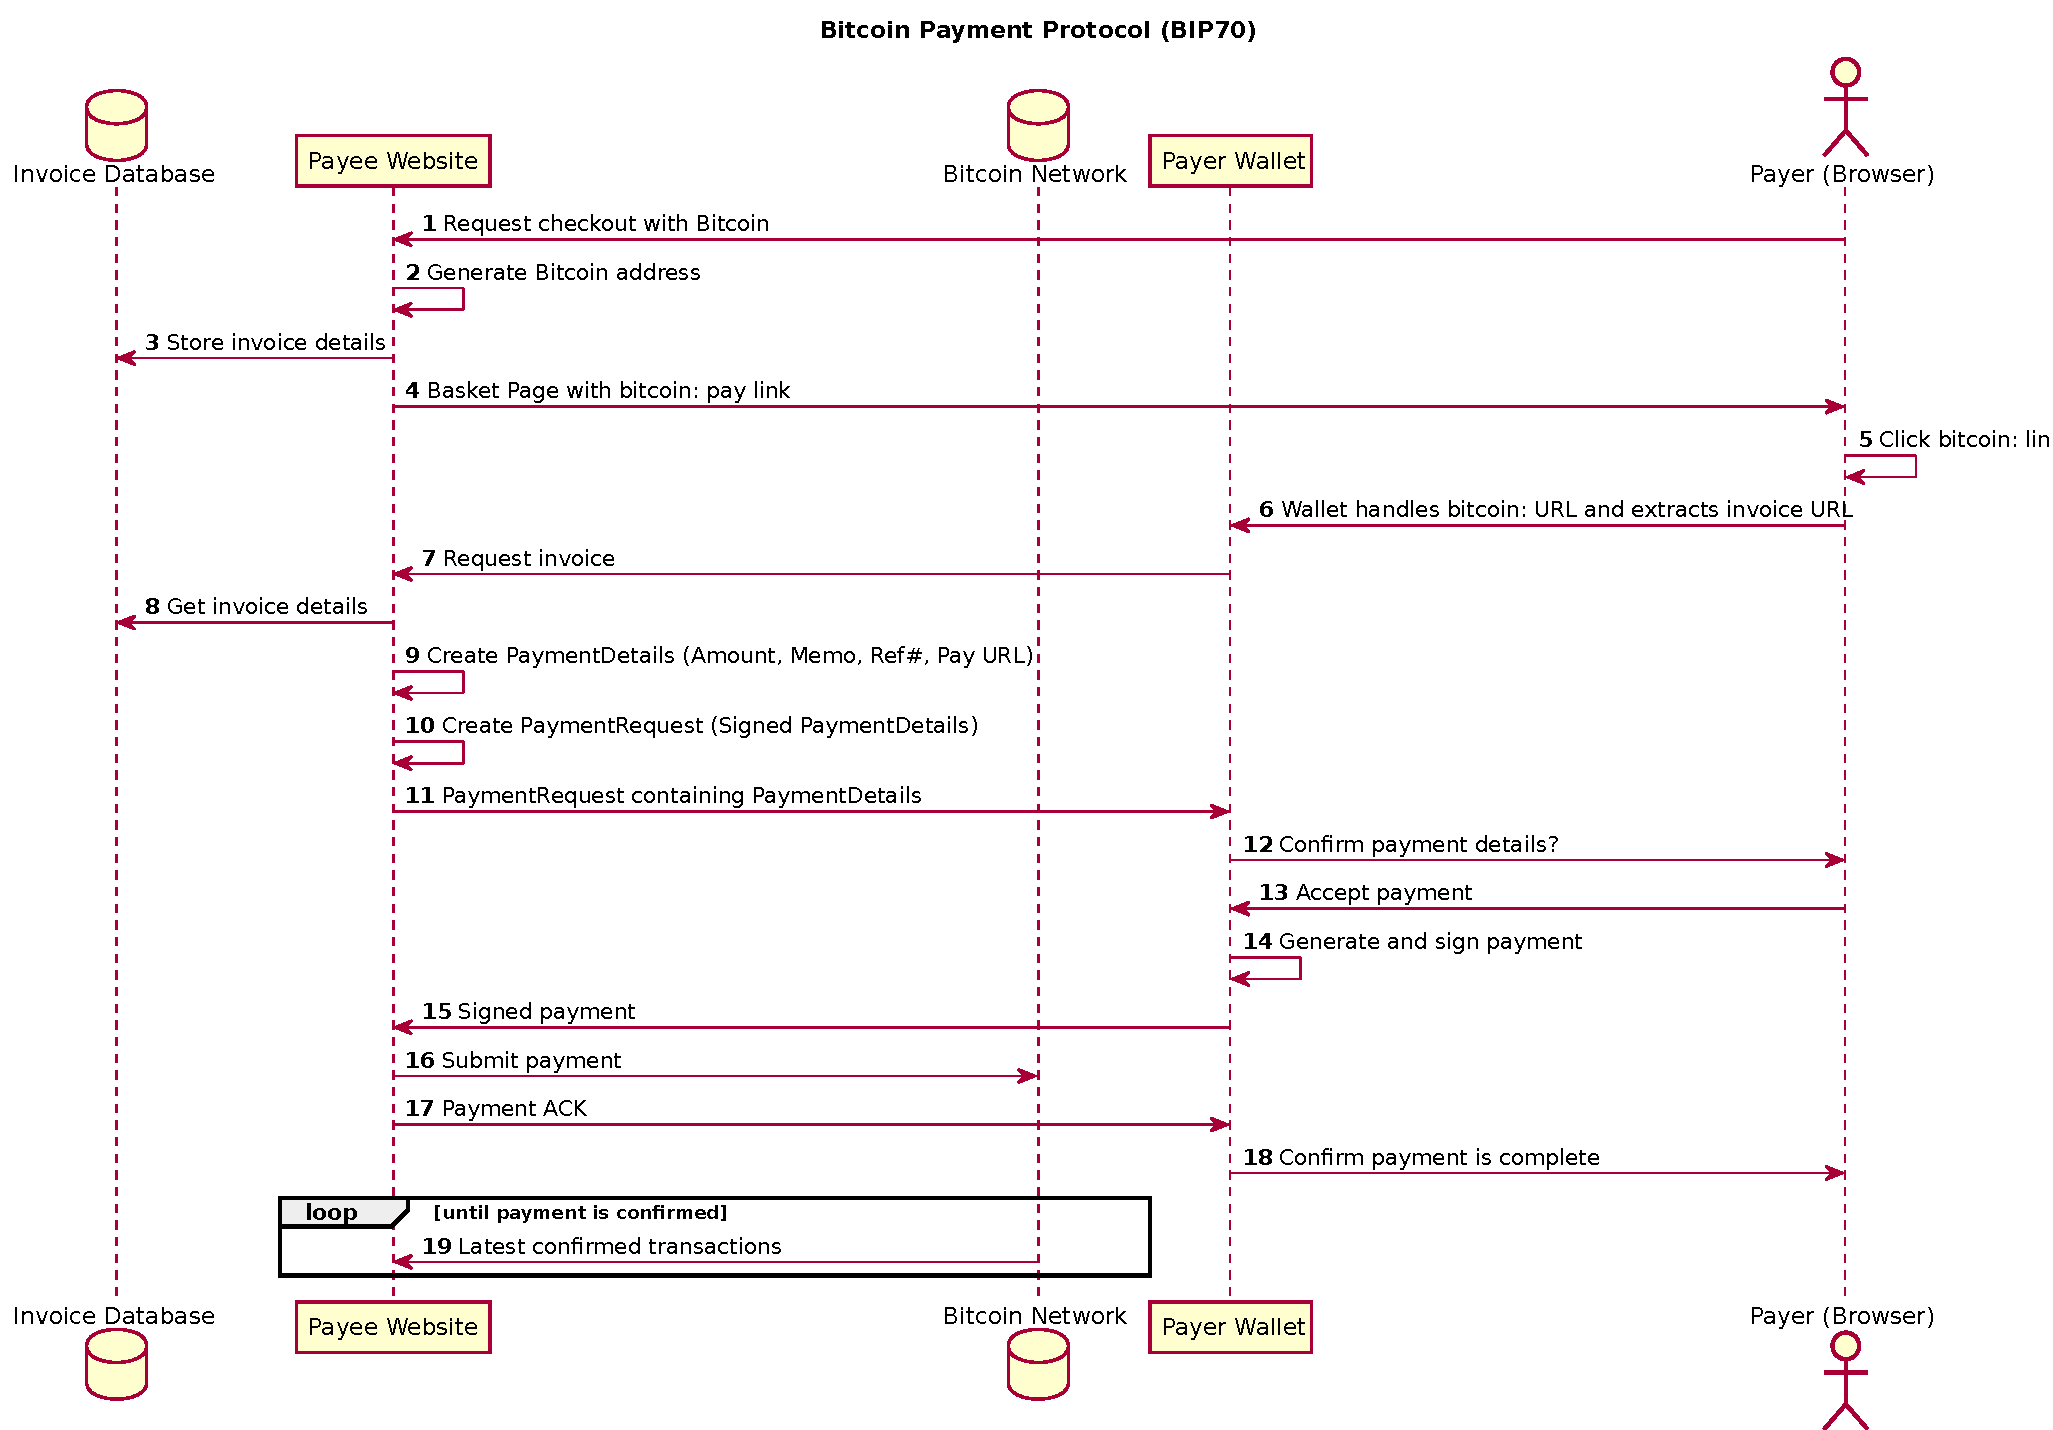
\includegraphics[width=\textwidth]{figs/bitcoin.pdf}
\caption{Bitcoin payment processing. (From: W3c Web Payments IG.)}
\label{fig:bitcoin}
\end{figure*}

% \tinyskip
\lstdefinelanguage{JavaScript}{
  keywords={typeof, new, true, false, catch, function, return, null, catch, switch, var, if, in, while, do, else, case, break, for},
  keywordstyle=\color{blue}\bfseries,
  ndkeywords={class, export, boolean, throw, implements, import, this},
  ndkeywordstyle=\color{darkgray}\bfseries,
  identifierstyle=\color{black},
  sensitive=false,
  comment=[l]{//},
  morecomment=[s]{/*}{*/},
  commentstyle=\color{purple}\ttfamily,
  stringstyle=\color{red}\ttfamily,
  morestring=[b]',
  morestring=[b]"
}

\begin{figure*}
 \lstset{language=JavaScript}
 \lstinputlisting{figs/taler-presence.js}
 \caption{Sample code to detect the Taler wallet. Allowing the
  Web site to detect the presence of the wallet leaks one bit
  of information about the user. The above logic also works
  if the wallet is installed while the page is open.}
  \label{listing:presence}
\end{figure*}


\begin{figure*}
 \lstset{language=JavaScript}
 \lstinputlisting{figs/taler-contract.js}
 \caption{Sample code to pass a contract to the Taler wallet.
          Here, the contract is fetched on-demand from the server.
          The {\tt taler\_pay()} function needs to be invoked
          when the user triggers the checkout.}
 \label{listing:contract}
\end{figure*}


\begin{figure*}
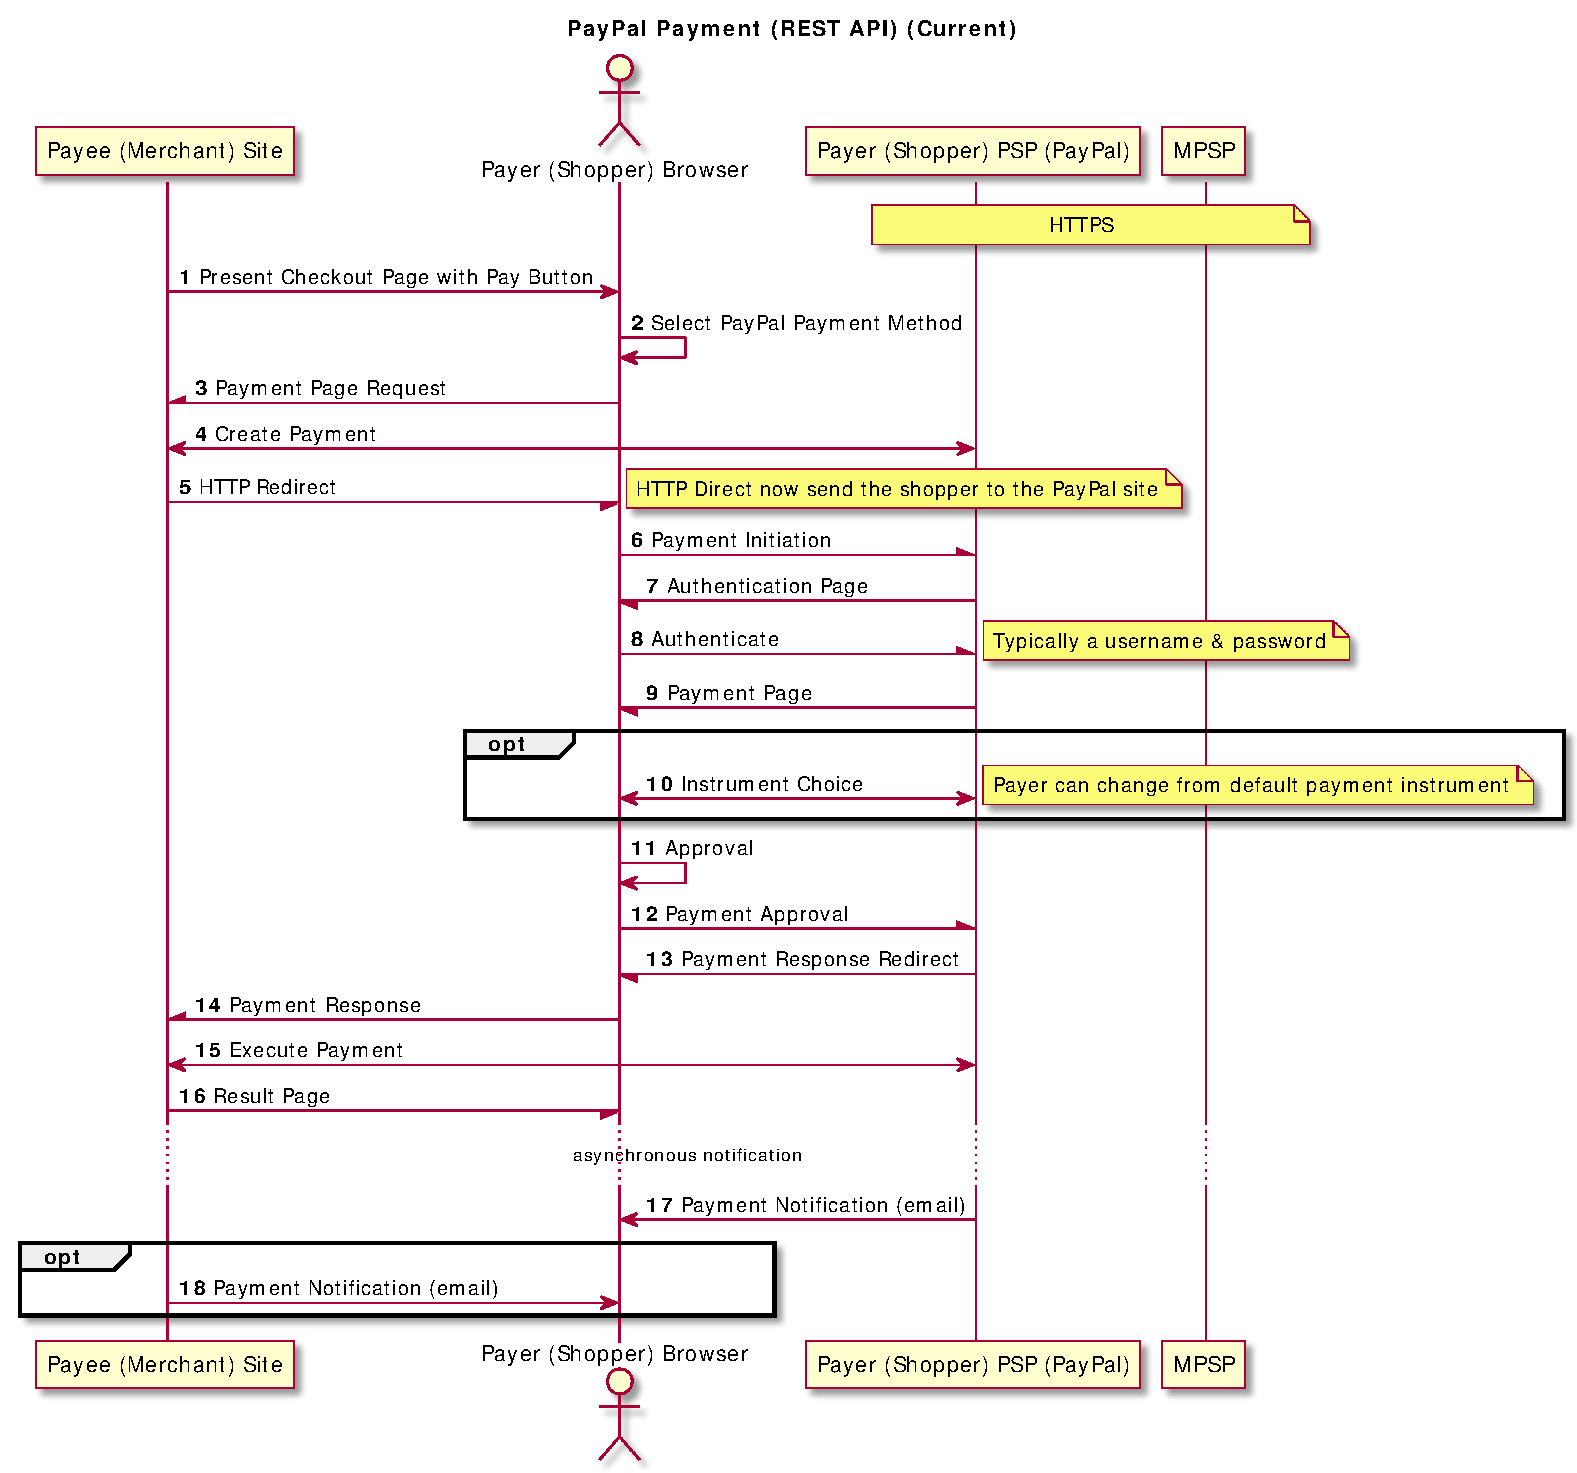
\includegraphics[width=\textwidth]{figs/paypal.pdf}
\caption{Payment processing with Paypal. (From: W3c Web Payments IG.)}
\label{fig:paypal}
\end{figure*}

\end{document}







% \smallskip
\subsection{Anonymity}

We strongly recommend that the user use Tor Browser to protect their
% FIXME wasn't the use of Tor discouraged to login into personal things?
IP address, both initially when withdrawing coins and later during
purchases.

There are lingering risks that anonymous coins can be correlated to
customers using additional information.

After withdrawing coins, customer should usually wait before spending
them, as spending them immediately ....
% wallet determines coin denominations







Wallet provides isolation
  Near copy from EXIST proposal?
- Limits user risk
- Nearly eliminates risk for merchant and exchange
  - lower transaction fees
- Reserves simplify things

Denomination choice
- Anonymity refresh protocol
- Withdraw automates like ATMs

Browser extension
- RESTful vs Bitcoin, OpenCoin, etc.
  - Retrying RESTful transactions always works
- minimizing dialog
- see & pay ??
- TBB integration
  - Needed anyways
- Other browser integration?
  - Is it wise?  Ok if not worried about anonymity  Taler is still better
  - Is tor2web worse?
- W3C

Autopay?  pat payment recognition?
- dangerous?
- high charges
- good for funny money

NFC













% \smallskip
\subsection{Risks}

A Taler exchange's need not face significant financial risks beyond
the risk of losing a denomination signing key.  Exchanges can limit that
risk by carefully tracking how much they issue in each denomination.
Taler merchant's risks are limited primarily by depositing coins
quickly and stating contracts accurately.
